\documentclass[11pt,a4paper]{article}
\usepackage[utf8]{inputenc}
\usepackage{hyperref}
\usepackage{tikz}
\usepackage{graphicx}
\usepackage{minted}
\usepackage{xcolor}

\usetikzlibrary{decorations.pathreplacing}
\setmintedinline{breaklines}
\setminted{breaklines}

\renewcommand{\figurename}{Figur}

\newcommand{\warning}[1]{
\noindent
\fbox{
\begin{minipage}{0.1\linewidth}
\raisebox{-6em}{
\scalebox{3}{%
\makebox[2.1em][c]{%
\makebox[0pt][c]{\raisebox{0.3em}{\large!}}%
\makebox[0pt][c]{\color{red}\Huge$\bigtriangleup$}}}
}
\end{minipage}
\begin{minipage}{0.1\linewidth}
\hfill
\end{minipage}
\begin{minipage}{0.7\linewidth}
\vspace{1em}
#1
\vspace{1em}
\end{minipage}
\begin{minipage}{0.05\linewidth}
\hfill
\end{minipage}
}
}

\title{Mikrokontrollerlab med micro:bit}
\author{TTK4235 Tilpassede Datasystemer}
\date{}

\begin{document}
\maketitle
\section{Bakgrunn}
\subsection{Introduksjon til micro:bit}
BBC micro:bit er et lite kort utviklet primært for å vekke interesse for programmering hos barn. For å gjøre dette mulig har man også laget et særs vennlig webgrensesnitt der man kan programmere kortet, simpelthen ved å trekke og slippe "programmeringsklosser" der man vil. Dette er selvsagt ideelt for å vise små barn at vi kan ha det gøy på Kyb, men utover dette får vi ingen kontroll over hva som skjer på et lavere nivå enn nettleseren.\\
\\
Litt lengre ned på abstraksjonsstigen har vi micro:bit DAL (Device Abstraction Layer). Denne kan programmeres via MicroPython eller JavaScript, men dette vil samtidig spise opp mye av ressursene tilgjengelig på det lille kortet. Eksempelvis vil man typisk kun ha omlag 2 KB SRAM-område tilgjengelig hvis man benytter seg av MicroPython; av de 16 KB kortet i utgangspunktet har.\\
\\
For å få en mer effektiv bruk av ressursene er det også mulig å benytte seg av C++, eksempelvis via ARM sin mbed-platform. Allikevel vil de fleste detaljene om hvordan kortet fungerer være abstrahert bort, også på dette nivået.\\
\\
For å få en bedre forståelse for hvordan en micro:bit fungerer, skal vi derfor fjerne DALen fra kortet og programmere prosessorens registre direkte. Prosessoren på kortet er en ARM Cortex M0, som er integrert inn i en Nordic Semiconductor nRF51822 SoC. Dette skal vi gjøre i C, som er det laveste abstraksjonsnivået vi kan få, uten å gå over til Thumb - som er prosessorens instruksjonssett.

\subsection{Introduksjon til labformatet}
Det finnes mange gode IDEer (Integrated Development Environments) for utvikling av innvevde datasystemer. Eksempelvis Keil, Atmel Studio, IAR Workbench, eller Segger Embedded Studio. Disse har en tendens til å koste en god del om man skal gjøre seriøs utvikling, og gjemmer dessuten mange detaljer for brukeren.\\
I denne laben vil vi derfor bruke ARM GCC som vår verktøykjede. Denne er det man kaller åpen kilde, og er helt uten begrensninger. For å ikke drukne dere i detaljer om hva som skjer i bakgrunnen, har vi allikevel laget en Makefil for dere. Denne vil bygge kildekoden for dere, sette opp riktig minnefordeling på prosessoren, og deretter skrive koden til den.\\
\\
I mappen dere har fått utdelt ligger det en gjemt undermappe ved navn ".build\_system". Denne inneholder det som skal til for å få koden deres til å kjøre på micro:biten. Det er ikke meningen at dere skal endre noe i denne mappen, men om dere vil forstå hvordan koden deres henger i hop med hva som skjer på kortet, er det bare å ta en titt.\\
\\
I bunnen av hver oppgavebeskrivelse vil det være hint til oppgaven. Dette kan være nyttig om dere står fast.

\subsubsection{Makefil}
For å bruke Makefilen, kaller dere \mintinline{bash}{make} fra et terminalvindu i samme mappe som Makefilen. Dette vil kompilere koden, og gjøre den om til en ".hex"-fil som mikrokontrolleren kan kjøre.\\
\\
Når dette er gjort, kan dere laste hex-filen over i programminnet til mikrokontrolleren. Dette gjøres ved å kalle \mintinline{bash}{make flash}.\\
\\
I tillegg til disse målene, har denne Makefilen også to andre mål; \mintinline{bash}{make erase} vil slette minnet til mikrokontrolleren, mens \mintinline{bash}{make clean} vil slette ferdigkompilert kode og hex-filen fra datamaskinen.


\subsubsection{Programmeringstaktikk}
For å sette ønskede registre på nRF51822en, vil vi bruke et kjent triks fra C-programmering; vi vil lage structer som dekker nøyaktig det minnet vi ønsker å fikle med - og så typecaste en peker til starten av minnet inn i structen. Dermed kan vi endre structens medlemsvariabler, og samtidig skrive til det underliggende minnet.

\subsection{Datablad}
Innvevde datasystemer er ganske forskjellige fra "vanlige" datasystemer, fordi de er skreddersydde for en spesifikk oppgave. Ofte må de fungere med begrensede ressurser, og gjerne over lang tid kun drevet av et knappecellebatteri. Derfor må vi glemme en del generelle ting som gjelder uavhengig av plattform, og fokusere på ting som kun gjelder plattformen vi arbeider på. Det er her datablad kommer inn.\\
\\
Datablad er tung, kortfattet, teknisk dokumentasjon som beskriver nøyaktig hvordan arkitekturen vi har brukes. Å finne frem i datablad er en egen kunst i seg selv.\\
\\
Gjennom dette emnet vil \href{http://infocenter.nordicsemi.com/pdf/nRF51\_RM\_v3.0.pdf}{\textbf{nRF51 Series Reference Manual}}\footnote{http://infocenter.nordicsemi.com/pdf/nRF51\_RM\_v3.0.pdf} stort sett være databladet vi skal bruke. Dette er et godt datablad som også er forholdsvis kort (datablad kan lett bli over tusen sider), så det er en god introduksjon til måten man jobber med innvevde systemer.

\section{Førstegangsoppsett}
Aller først må vi sette opp de redskapene vi trenger for å kunne programmere micro:biten som vi vil. Seksjon \ref{sec::setup::software} setter opp verktøykjeden på datamaskinen, mens seksjon \ref{sec::setup::hardware} dekker hvordan dere klargjør micro:biten.

\subsection{Software}
\label{sec::setup::software}
På Sanntidssalen vil nok dette steget være gjort for de fleste av dere, men dersom dere har lyst til å programmere micro:biten utenfor labtidene, vil denne seksjonen gi en generell oppskrift for hvordan dere kan gjøre det.\\
\\
For å se om alle verktøyene er på plass før vi starter, kan dere kalle \mintinline{bash}{nrfjprog --version} fra kommandolinjen. Om denne kommandoen svarer med en versjon for både \mintinline{text}{nrfjprog} og \mintinline{text}{JLinkARM}, trenger dere ikke gjøre noe her.

\subsubsection{arm-none-eabi-gcc}
Kompilatoren vi skal bruke er GCC for ARM. På Linuxmaskiner finnes denne utvidelsen for GCC gjerne i systempakkelageret. På Ubuntu installeres denne enkelt ved å kalle
\begin{minted}{bash}
sudo apt install gcc-arm-none-eabi
\end{minted}

\subsubsection{nrfjprog}
For å laste ferdigkompilert kode over på micro:biten skal vi bruke Nordic sitt flasheverktøy - \mintinline{text}{nrfjprog}. Dette installerer dere slik:
\begin{enumerate}
\item Gå til \href{infocenter.nordicsemi.com}{infocenter.nordicsemi.com}.
\item Under \mintinline{text}{nRF Tools} velger dere \mintinline{text}{nRF5x Command Line Tools}, og så \mintinline{text}{Installing the nRF5x Command Line Tools}.
\item Velg nedlastingen for Linux 64-bit. Dette vil ta dere til en side hvor dere kan laste ned siste versjon av verktøyet.
\item Når dere har lastet ned \mintinline{text}{.tar}-filen, navigerer dere til mappen dere lastet den ned til, via terminalen.
\item Brett ut tararkivet ved å kalle \mintinline{bash}{tar -xf nRF5x-Com[...]x86_64.tar}
\item Kall så \mintinline{bash}{sudo chown root:root -R nrfjprog}. Dette vil gi eierskap over mappen \mintinline{text}{nrfjprog} til rotbrukeren.
\item Kall deretter \mintinline{bash}{sudo mv nrfjprog/* /usr/bin}. Dette vil flytte alt innholdet i nrfjprogmappen inn i \mintinline{text}{/usr/bin} - som er et sted inkludert i miljøvariabelen \mintinline{text}{$PATH}%$
. Det betyr simpelthen at dere kan kjøre programmet fra hvor som helst uten å måtte spesifisere hvor det ligger.
\end{enumerate}

\subsubsection{JLinkARM}
Til slutt må \mintinline{text}{nrfjprog} vite hvordan det skal snakke med programvaren på micro:biten. Etter seksjon \ref{sec::setup::hardware}, vil denne programvaren være JLink, så vi må her finne ut hvordan vi får \mintinline{text}{nrfjprog} til å snakke JLink.
\begin{enumerate}
\item Gå til \href{segger.com/downloads/jlink}{segger.com/downloads/jlink}.
\item Under \mintinline{text}{J-Link Software and Documentation Pack}, finner dere alternativet \mintinline{text}{DEB installer 64-bit}.
\item Velg \mintinline{text}{Older versions}, fordi versjon \textbf{V6.30f} i skrivende stund har en bug der dere mister forbindelse med micro:biten hver gang dere kjører \mintinline{text}{nrfjprog}.
\item Velg versjon \textbf{V6.30} (altså uten noen bokstav bak).
\item Via terminalen, gå til mappen dere lastet ned til.
\item Kall \mintinline{bash}{sudo dpkg -i JLink_Linux[...]x86_64.deb}
\end{enumerate}
Til slutt kan dere nå kalle \mintinline{bash}{nrfjprog --version} igjen, for å se om alt er installert riktig.

\subsection{Hardware}
\label{sec::setup::hardware}
Før vi kan programmere micro:biten må vi kvitte oss med DALen. Last ned \href{https://www.segger.com/downloads/jlink\#BBC_microbit}{BBC micro:bit J-Link OB Firmware}\footnote{www.segger.com/downloads/jlink\#BBC\_microbit} fra Segger.com. Dette er en hex-fil som vi skal legge inn på micro:biten for å få tilgang til programmering via Nordics flashverktøy, \textbf{nrfjprog}, og bedre debuggingsmuligheter enn vi har fra før.

\begin{enumerate}
\item Hold inne Reset på micro:biten. Dette er knappen på siden med logoen til micro:bit. Mens knappen holdes inne, koble inn USBen.
\item Det skal nå komme opp en enhet med navn "MAINTENANCE" på datamaskinen. Nå kan Reset slippes.
\item Trekk hex-filen fra Segger inn i "MAINTENANCE".
\item Etter at hex-filen er ferdig overført, vil micro:biten automatisk tilkobles på nytt. Denne gangen som "MICROBIT".
\item Kjør kommandoen \mintinline{bash}{nrfjprog -f nrf51 -e} fra terminalen.
\item LED-matrisen skal nå slutte å lyse.
\end{enumerate}

\section{Oppgave 1: GPIO}
\subsection{Beskrivelse}
I denne laben skal vi skru på alle LEDene i matrisen når knappen "B" trykkes, og skru dem av når knappen "A" trykkes.\\
\\
Denne laboppgaven vil være litt kokebok, for å introdusere noen konsepter dere skal bruke senere. Deretter vil det bli gradvis mindre håndholding. Det kan være lurt å skumme gjennom appendikset for en rask oppsummering av hvordan vi gjør bitoperasjoner i C.\\
\\
LED-matrisen på micro:biten er implementert litt annerledes enn det man kanskje tror. Istedenfor å bruke en 5x5 matrise direkte, har man implementert den som en 3x9 matrise der to av cellene ikke er koblet til en diode. Dette er illustrert i figur \ref{fig::microbit::ledmatrix}. I denne matrisen er pinne 4 til pinne 12 jord, mens pinne 13 til pinne 15 er strømforsyning. Dermed, for å få diode nummer 12 til å lyse, må P6 være trukket lav, mens P14 være høy.

\begin{figure}
\centering
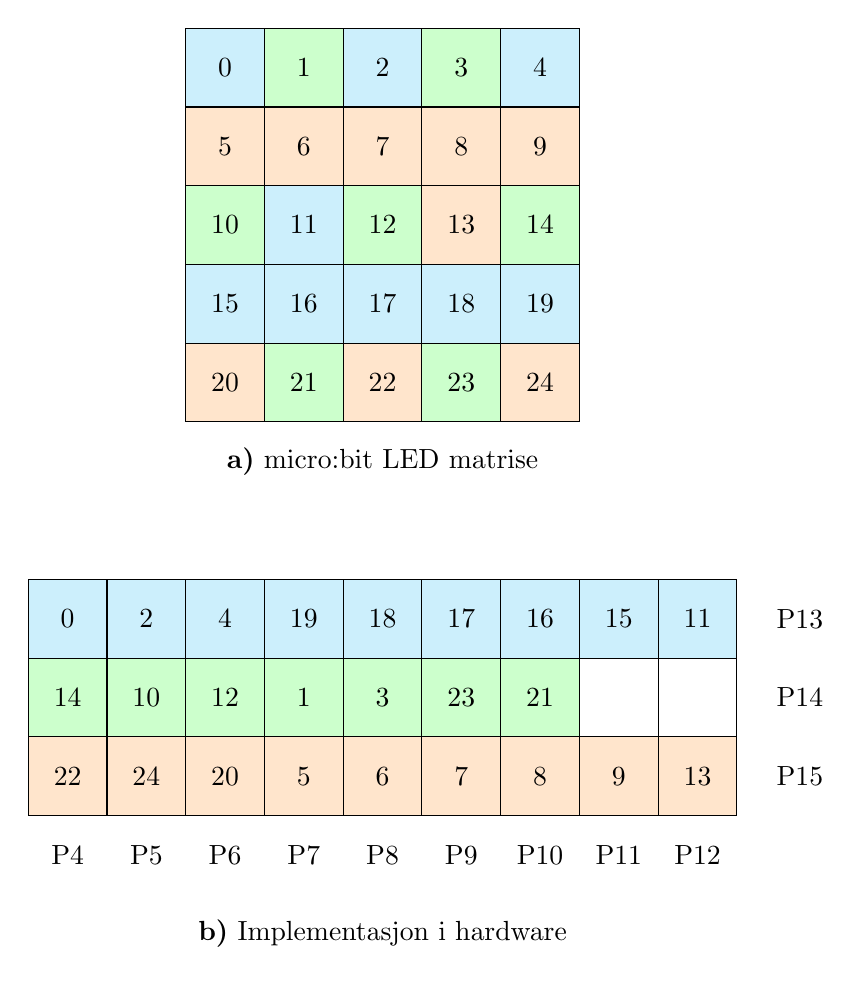
\begin{tikzpicture}
\colorlet{PRI}{cyan!20}
\colorlet{SEC}{green!20}
\colorlet{TRT}{orange!20}

% Physical LED matrix
\foreach \x/\f in {0/PRI,1/SEC,2/PRI,3/SEC,4/PRI}{
	\fill[\f] (\x,4) rectangle ++(1,1);
}
\foreach \x in {0,1,...,4}{
	\fill[TRT] (\x,3) rectangle ++(1,1);
}
\foreach \x/\f in {0/SEC,1/PRI,2/SEC,3/TRT,4/SEC}{
	\fill[\f] (\x,2) rectangle ++(1,1);
}
\foreach \x in {0,1,...,4}{
	\fill[PRI] (\x,1) rectangle ++(1,1);
}
\foreach \x/\f in {0/TRT,1/SEC,2/TRT,3/SEC,4/TRT}{
	\fill[\f] (\x,0) rectangle ++(1,1);
}

\foreach \x in {0,1,...,4}{
\foreach \y in {0,1,...,4}{
	\pgfmathtruncatemacro{\result}{\x + (4 - \y)*5}
	\draw (\x,\y) rectangle ++(1,1) node [midway] {\result};
}
}

\path (0,-1) rectangle ++(5,1) node [midway] {\textbf{a)} micro:bit LED matrise};

% Hardware implemented LED matrix
\begin{scope}[xshift=-2cm,yshift=-5cm]
\foreach \x/\num in {0/0,1/2,2/4,3/19,4/18,5/17,6/16,7/15,8/11}{
	\draw[fill=PRI] (\x, 2) rectangle ++(1,1) node [midway] {\num};
}
\foreach \x/\num/\f in {0/14/SEC,1/10/SEC,2/12/SEC,3/1/SEC,4/3/SEC,5/23/SEC,6/21/SEC,7//white,8//white}{
	\draw[fill=\f] (\x, 1) rectangle ++(1,1) node [midway] {\num};
}
\foreach \x/\num in {0/22,1/24,2/20,3/5,4/6,5/7,6/8,7/9,8/13}{
	\draw[fill=TRT] (\x, 0) rectangle ++(1,1) node [midway] {\num};
}
\foreach \x in {0,1,...,8}{
	\pgfmathtruncatemacro{\pin}{\x + 4}
	\path (\x,-1) rectangle ++(1,1) node [midway] {P\pin};
}
\foreach \y/\pin in {2/13,1/14,0/15}{
	\path (9.3,\y) rectangle ++(1,1) node [midway] {P\pin};
}

\path (0,-2) rectangle ++(9,1) node [midway] {\textbf{b)} Implementasjon i hardware};

\end{scope}

\end{tikzpicture}
\caption{Utseende av- versus implementasjon av micro:bit LED matrise.}
\label{fig::microbit::ledmatrix}
\end{figure}

\subsection{Oppgave}
Ta en titt på den vedlagte filen "schematics.pdf"; dette er referansedesignet for en micro:bit. Finn ut hvordan de to knappene er koblet. Hvilke pinner på nRF51822en brukes? Vil pinnene være høye eller lave dersom knappene trykkes?\\
\\
Se deretter i databladet til nRF51-serien. Hvordan ser minnekartet for mikrokontrolleren ut? Hva er baseadressen til GPIO-modulen? Bytt ut \mintinline{c}{__GPIO_BASE_ADDRESS__} i mainfilen med den faktiske baseaddressen.\\
\\
I mainfilen vil dere se at det er definert en struct ved navn \mintinline{c}{NRF_GPIO_REGS}. Denne structen representerer alle registrene til GPIO-modulen. Ved å \textit{typecaste} adressen til GPIO-modulen inn i structen, kan vi så endre på structens medlemsvariabler for å skrive til registrene. Det er nettopp dette som er formålet med kodelinjen
\begin{minted}{c}
#define GPIO ((NRF_GPIO_REGS*)__GPIO_BASE_ADDRESS__)
\end{minted}
Når denne er definert, kan vi eksempelvis endre \mintinline{c}{OUT}-registret ved å kalle
\begin{minted}{c}
GPIO->OUT = desired_value;
\end{minted}
Dere vil også se at medlemsvariabelen \mintinline{c}{RESERVED0} er en array av type \mintinline{c}{volatile uint32_t} med 321 elementer. Dette er fordi databladet forteller oss at \mintinline{c}{OUT}-registeret har en offset på 0x504 ($504_{16}$) fra GPIO-modulens baseadresse. $504_{16}$ er det samme som $1284_{10}$. Altså er det 1284 byte mellom baseadressen og \mintinline{c}{OUT}-registeret. Siden vi bruken en ordstørrelse på 32 bit, deler vi dette tallet på fire, ettersom 32 bit er 4 byte. Dermed har vi $1284 / 4 = 321$.\\
\\
Ved å følge samme resonnement, hva skal da \mintinline{c}{__RESERVED1_SIZE__} være? Finn ut dette, og endre mainfilen tilsvarende.\\
\\
Når dere har gjort det, kan dere fylle ut de manglende bitene av \mintinline{c}{main()}, slik at LED-matrisen lyser når vi trykker knapp B, og skrur seg av når vi trykker knapp A.

\subsection{Hint}
\begin{enumerate}
\item nRF51822 har en GPIO-modul, og en GPIOTE-modul (\textbf{G}eneral \textbf{P}urpose \textbf{I}nput/\textbf{O}utput \textbf{T}asks and \textbf{E}vents). Sistnevnte brukes for å lage et hendelsesbasert system. Vi skal i første omgang kun bruke GPIO-modulen.
\item Om dere skriver inn GPIO-modulens baseadresse i base 16 (hexadecimal), må dere huske "0x" foran adressen. Hvis ikke vil kompilatoren tro dere mener base 10.
\item Når dere skal finne \mintinline{c}{__RESERVED1_SIZE__}, så husk at \mintinline{c}{DIRCLR} starter på 0x51C, som betyr at den byten slutter på 0x51F. Altså så starter ikke \mintinline{c}{RESERVED1} på 0x51C, men på 0x520.
\end{enumerate}

\section{Oppgave 2: UART}
\subsection{Beskrivelse}
I denne oppgaven skal vi sette opp toveis kommunikasjon mellom datamaskinen og micro:biten. Dette skal vi gjøre ved å bruke UART, som står for \textbf{U}niversal \textbf{A}synchronous \textbf{R}eceiver-\textbf{T}ransmitter. Tradisjonelt ble signalene sent mellom to UART-moduler båret over et RS232 COM grensesnitt. Nå har det seg derimot slik at moderne datamaskiner ikke lages med en slik port. Labdatamaskinene på Sanntidssalen har en DSUB9-port, som vi kunne brukt, men i dette tilfellet er vi heldigere enn som så.\\
\\
Om dere ser etter på micro:biten, vil dere se en liten chip med nummer M26M7V. Dette er faktisk en ekstra Freescale MKL26Z128VFM4 mikrokontroller. Grunnen til at denne er der, er først og fremst at den lar oss programmere nRF51822-SoCen over USB. I tillegg til dette implementerer den en USB CDC (\textbf{C}ommunications \textbf{D}evice \textbf{C}lass), som lar oss "pakke inn" UART-signaler i USB-pakker. På den måten vil datamaskinen se ut som en UART-enhet for mikrokontrolleren; og mikrokontrolleren vil se ut som en USB-enhet for datamaskinen.

\subsection{Kort om UART på nRF51 og micro:bit}
Modulen for UART som finnes på nRF51822-SoCen implementerer såkalt \textit{full duplex} med automatisk flytkontroll. Full duplex betyr simpelthen at UARTen er i stand til å både sende- og motta meldinger samtidig. For å tillate full duplex, trengs det naturlig nok en dedikert linje for å motta; og en dedikert linje for å sende. Flytkontrollen består av to ekstra linjer, som brukes for å avtale når en enhet kan sende, og når den må holde kjeft.\\
\\
Dermed er vi totalt oppe i fire linjer: \mintinline{text}{RXD} (Mottakslinje), \mintinline{text}{TXD} (Sendelinje), \mintinline{text}{CTS} (\textbf{C}lear \textbf{T}o \textbf{S}end), og \mintinline{text}{RTS} (\textbf{R}equest \textbf{T}o \textbf{S}end). Når alle disse linjene brukes, er det mulig å oppnå en pålitelig overføringshastighet på 1 million bit per sekund. Dette er ganske imponerende med tanke på at "vanlig" UART-hastighet ligger på 115200 bit per sekund.\\
\\
Uheldigvis er ikke alt bare fryd og gammen, rett og slett fordi vi blir tvunget til å snakke gjennom Freescalechipen om vi ønsker å kunne tolke signalet som USB. Grunnen til at dette er problematisk, er at micro:biten bare kobler to UART-linjer mellom de to chipene, så vi må holde oss til UART uten flytkontroll. Dette betyr at den høyeste baudraten vi pålitelig kan sende med, er 9600 bit per sekund. Stort sett vil micro:biten kunne håndtere høyere rater enn dette, men om dere ønsker minimalt med pakketap, er det lurt å holde seg til 9600 baud. Forutsatt at dere setter pakkestørrelsen til 8 bit, og bruker 2 stoppbit, vil dette uansett gi dere en overføringshastighet på omlag 800 bokstaver per sekund - som burde være mer enn nok.

\subsubsection{Noe å ha i bakhodet}
På nRFen er det nyttig å tenke på UARTmodulen som en tilstandsmaskin, der den vil sende så lenge den er i tilstanden \mintinline{text}{STARTTX}. Den vil bare stoppe å sende når den forlater denne tilstanden, altså når den går over i \mintinline{text}{STOPTX}. Dette er veldig godt illustrert i figur 68 i referansemanualen.

\subsection{Oppgave}
Det første vi må gjøre, er å identifisere hvor UART-pinnene er koblet. Både nRF51- og nRF52-serien er i stand til å koble hver enkelt modul til et vilkårlig sett av GPIO-pinner, så om vi designet kretsen selv, hadde dette vært opp til oss.\\
Slik er det altså ikke, så vi må ta en titt i "schematics.pdf". Finn ut hvilken pinne fra nRF51822-chipen som er \mintinline{c}{TGT_RXD}, og hvilken pinne som er \mintinline{c}{TGT_TXD}. Disse pinnene skal vi sene konfigurere som henholdsvis input og output.\\
\\
Opprett nå filene "uart.h" og "uart.c". Headerfilen skal inneholde deklarasjonen til tre funksjoner:
\begin{minted}{c}
void uart_init();
void uart_send(char letter);
char uart_read();
\end{minted}
Denne headerfilen inkluderes fra mainfilen. I implementasjonsfilen ("uart.c") skal vi igjen bruke en struct til minneoperasjoner, slik vi gjorde for GPIO:
\begin{minted}{c}
#include <stdint.h>

#define UART ((NRF_UART_REG*)0x--------)

typedef struct {
	volatile uint32_t ...;
} NRF_UART_REG;
\end{minted}
Dere må også legge til "uart.c" bak \mintinline{c}{SOURCES := main.c} i Makefilen, slik at kompilatoren kompilerer denne filen også.

\subsubsection{\texorpdfstring{\mintinline{c}{void uart_init()}}{void uart\_init()}}
Denne funksjonen skal først konfigurere de nødvendige GPIO-pinnene som input/output. Derfor må "gpio.h" inkluderes i "uart.c". Denne filen er allerede skrevet for dere.\\
\\
Når pinnene er konfigurert i GPIO-modulen, må de brukes av UART-modulen. Dette gjøres via \mintinline{c}{PSELTXD}- og \mintinline{c}{PSELRXD}-registrene.\\
\\
Om dere ser i "schematics.pdf", vil dere se at vi ikke har noen CTS- eller RTS-koblinger fra nRF51-chipen (\textbf{C}lear \textbf{T}o \textbf{S}end og \textbf{R}equest \textbf{T}o \textbf{S}end). Dette betyr at vi ikke er i stand til å gjøre flytkontroll i hardware. Dermed står vi i fare for å miste pakker om vi prøver å sende for fort. Velg derfor en baudrate på 9600. "Baudrate" forteller simpelthen hvor mange bit vi sender per sekund.\\
Av samme grunn må vi fortelle UART-modulen at vi ikke har CTS- og RTS-linjer. Sett opp de riktige registrene for dette.\\
\\
Til slutt skal vi gjøre to ting. Først må vi skru på UART-modulen, som gjøres via et eget \mintinline{c}{ENABLE}-register. Deretter skal vi starte å ta imot meldinger, sett derfor \mintinline{c}{STARTRX} til 1.

\subsubsection{\texorpdfstring{\mintinline{c}{void uart_send(char letter)}}{void uart\_send(char letter)}}
Denne funksjonen skal ta i mot én enkel bokstav, å sende den over til datamaskinen. Ta en titt på figur 68 ("UART Transmission") i databladet til nRF51-serien for å finne ut hva dere skal gjøre. Husk å vente til sendingen er ferdig, før dere skrur av sendefunksjonaliteten.

\subsubsection{\texorpdfstring{\mintinline{c}{char uart_read()}}{char uart\_read()}}
Denne funksjonen skal lese én bokstav fra datamaskinen og returnere den. Vi ønsker ikke at funksjonen skal blokkere, så om det ikke er en bokstav klar akkurat når den kalles, skal den returnere \mintinline{c}{'\0'}.\\
\\
Husk at dere må gjøre dette i en bestemt rekkefølge for å kunne garantere at UART-modulen ikke taper informasjon. Det vil si, sett \mintinline{c}{RXDRDY} til 0 før dere leser \mintinline{c}{RXD} - og sørg også for å kun lese \mintinline{c}{RXD} én gang.\\
\\
Dere skal ikke skru av mottakerregisteret når dere har lest meldingen.
\subsection{Sendefunksjon}
Programmér micro:biten til å sende \mintinline{c}{'A'} om knappen A trykkes, og \mintinline{c}{'B'} om B trykkes. For å motta meldingene på datamaskinen, skal vi bruke programmet \mintinline{bash}{picocom}. Fra et terminalvindu, kaller dere:
\begin{minted}{bash}
picocom -b 9600 /dev/ttyACM0
\end{minted}
Dette vil fortelle \mintinline{bash}{picocom} at det skal høre etter enheten \mintinline{bash}{/dev/ttyACM0}, med baudrate 9600.\\
\\
Merk at den siste bokstaven bak "ACM" er et null-tegn.

\subsection{Mottaksfunksjon}
Lytt etter sendte pakker på micro:biten. Om datamaskinen har sendt en bokstav, skal micro:biten skru på LED-matrisen om den var av, og skru den av om den allerede var på. Husk at \mintinline{c}{char uart_read()} returnerer \mintinline{c}{'\0'} om ingenting var sendt.\\
\\
For å sende bokstaver fra datamaskinen bruker vi igjen \mintinline{bash}{picocom}. Standardoppførselen til \mintinline{bash}{picocom} er å sende alle bokstaver som skrives inn i terminalen når det kjører. Bokstavene vil derimot ikke bli skrevet til skjermen, så dere vil ikke få noen visuell tilbakemelding på datamaskinen (om dere ikke manuelt sender bokstaven tilbake fra micro:biten).

\subsection{Mer avansert IO}
Nå har dere en funksjon for å sende over nøyaktig én bokstav av gangen; og en funksjon for å motta nøyaktig én bokstav av gangen. Om vi ønsker å sende en C-streng av vilkårlig lengde kunne vi laget en funksjon som dette:
\begin{minted}{c}
void uart_send_str(char ** str){
	UART->STARTTX = 1;
	char * letter_ptr = *str;
	while(*letter_ptr != '\0'){
		UART->TXD = *letter_ptr;
		while(!UART->TXDRDY);
		UART->TXDRDY = 0;
		letter_ptr++;
	}
}
\end{minted}
Denne funksjonen vil fungere, men den er ikke annet enn en "dum" variant av \mintinline{c}{printf()}. Den gjør nemlig nesten det samme som \mintinline{c}{printf}, men den har ingen av formateringsalternativene som gjør \mintinline{c}{printf} ettertraktet.\\
\\
Vi vil heller inkludere \mintinline{c}{<stdio.h>} og bruke en heltallsvariant av \mintinline{c}{printf}, kalt \mintinline{c}{iprintf}. Nå har vi derimot ett problem: \mintinline{c}{printf} vil i utgangspunktet snakke med en strøm som heter \mintinline{c}{stdout}, som tradisjonelt sett peker til en terminal.\\
Mikrokontrolleren vår har ingen skjerm - og dessuten er ikke \mintinline{c}{printf} egentlig implementert ferdig for oss på denne plattformen. Dette er fordi vår variant av \mintinline{c}{<stdio.h>} kommer fra et bibliotek kalt \mintinline{c}{newlib} - som er skrevet spesielt for innvevde datamaskiner.\\
Når \mintinline{c}{printf(...)} kalles, vil et annet funksjonskall til \mintinline{c}{_write_r(...)} skje i bakgrunnen. Denne funksjonen vil deretter kalle \mintinline{c}{ssize_t _write(int fd, const void * buf, size_t count)}, som foreløpig ikke gjør noe. Grunnen til at denne finnes, er at den trengs for at programmet skal kompilere, men den er i utgangspunktet tom, fordi vi gir lenkeren flagget \mintinline{c}{--specs=nosys.specs}, som dere kan se i Makefilen.\\
\\
Gjennom \mintinline{c}{newlib} kan vi faktisk lage mange varianter av slike skrivefunksjoner, om vi har et komplekst innvevd system med mange skriveenheter, eller om vi har flere tråder. Denne arkitekturen har bare én kjerne - og vi vil bare bruke UART, så vi kan fint implementere en global variant av denne skrivefunksjonen. For å gjøre det, legger vi til følgene i mainfilen:
\begin{minted}{c}
#include <stdio.h>

[...]

ssize_t _write(int fd, const void *buf, size_t count){
	char * letter = (char *)(buf);
	for(int i = 0; i < count; i++){
		uart_send(*letter);
		letter++;
	}
	return count;
}
\end{minted}
Merk at returtypen til \mintinline{c}{_write} er \mintinline{c}{ssize_t}, mens \mintinline{c}{count}-variabelen er av type \mintinline{c}{size_t}. Når denne funksjonen er implementert, kan dere kalle \mintinline{c}{iprintf} fra programmet deres.\\
\\
Prøv å kalle \mintinline{c}{iprintf("Norway has %d counties.\n\r", 18)}. Om \mintinline{bash}{picocom} da forteller dere at Norge består av 18 fylker, så har dere greid oppgaven.

\subsection{\texorpdfstring{Frivillig: \mintinline{c}{_read()}}{Frivillig: \_read()}}
Vi kan også implementere funksjonen \mintinline{c}{ssize_t _read(int fd, void *buf, size_t count)}, slik at vi kan bruke \mintinline{c}{scanf} fra \mintinline{c}{<stdio.h>}. Legg til denne funksjonen i mainfilen:
\begin{minted}{c}
ssize_t _read(int fd, void *buf, size_t count){
	char *str = (char *)(buf);
	char letter;
	
	do {
		letter = uart_read();
	} while(letter == '\0');
	
	*str = letter;
	return 1;
}
\end{minted}
Skriv deretter et kort program som spør datamaskinen etter 2 heltall. Disse skal leses inn til micro:biten, som vil gange dem sammen, og sende resultatet tilbake til datamaskinen.

\subsection{Hint}
\begin{enumerate}
\item Det skal være totalt 11 reserverte minneområder i UART-structen. De skal ha følgene størrelser: 3, 56, 4, 1, 7, 110, 93, 31, 1, 1, 17.
\item Det er ingen forskjell på \textit{tasks}, \textit{events} og vanlige registre. Når LSB er satt i et \textit{event}-register, har en hendelse skjedd. Når LSB settes i et \textit{task}-register, startes en oppgave.
\item \mintinline{c}{int fd} i \mintinline{c}{_read} og \mintinline{c}{_write} står for "file descriptor". Den er der i tilfelle noen vil bruke \mintinline{c}{newlib} i forbindelse med et operativsystem. Vi trenger derimot ikke tenke på det.
\item Husk å legge til "uart.c" i Makefilen, bak \mintinline{c}{SOURCES : = main.c}.
\end{enumerate}

\section{Oppgave 3: GPIOTE og PPI}
\subsection{Beskrivelse}
Nå har det seg slik at vi jobber på en ganske ressursbegrenset plattform, som stort sett er tilfellet når vi driver med innvevde datasystemer. For eksempel er nRF51822 SoCen basert på en ARM Cortex M0, som bare har én kjerne. Derfor har vi ikke mulighet til å kjøre kode i sann parallell. Vi kan selvsagt bytte veldig fort mellom to eller flere \textit{fibre}, men dette vil skape en del problemer om vi trenger nøyaktige tidsverdier.\\
\\
For å løse dette problemet, har nRF51822en noe som kalles \textbf{P}rogrammable \textbf{P}eripheral \textbf{I}nterconnect. Dette er en teknologi som lar oss direkte koble en perifer enhet til en annen, uten at vi trenger å snakke med CPUen. For å dra nytte av denne teknologien må vi innføre \textit{oppgaver} og \textit{hendelser} - eller \textit{tasks} og \textit{events}. Oppgaver og hendelser er egentlig bare registre, men brukes annerledes enn "vanlige" registre.\\
Om et hendelsesregister inneholder verdien 1 har en hendelse inntruffet; om registeret inneholder verdien 0, har hendelsen ikke inntruffet. Oppgaveregistre er knyttet til en gitt oppgave (derav navnet), som kan startes ved å skrive verdien 1 til det. Oppgaver kan derimot ikke stanses ved å skrive verdien 0 til samme register som startet oppgaven.\\
\\
De fleste perifere enhetene som finnes på nRF51822 har noen form for oppgaver og hendelser. For å knytte oppgaver og hendelser til GPIO-pinnene, har vi en egen modul kalt GPIOTE - som står for \textbf{G}eneral \textbf{P}urpose \textbf{I}nput \textbf{O}utput \textbf{T}asks and \textbf{E}vents.\\
\\
I denne oppgaven skal vi bruke GPIOTE-modulen til å definere en hendelse (A-knapp trykket), og tre oppgaver (skru på eller av spenning til de tre LED-matriseforsyningene).

\subsection{Oppgave}
Først må jordingspinnene til LED-matrisen konfigureres som output, og settes til logisk lave. Dere trenger ikke konfigurere forsyningspinnene, fordi GPIOTE-modulen vil ta hånd om dette for dere. På samme måte slipper dere å konfigurere A-knappen som input.\\
\\
Dere har allerede fått utlevert headerfilene "gpiote.h" og "ppi.h", men dere må selv lese kapitlene om GPIOTE og PPI for å se hvordan de skal brukes. Når dere har gjort det, skal dere gjøre følgende:

\subsection{GPIOTE}
Alle de fire GPIOTE-kanalene skal brukes. Bruk én kanal til å lytte til A-knappen. Denne kanalen skal generere en hendelse når knappen trykkes - altså når spenningen på GPIO-pinnen går fra høy til lav.\\
\\
De tre resterende kanalene skal alle være konfigurert som oppgaver, og koblet til hver sin forsyningspinne for LED-matrisen. Forsyningsspenningen skal veksle hver gang oppgaven aktiveres. Hvilken initialverdi disse GPIOTE-kanalene har, er opp til dere.

\subsection{PPI}
For å koble A-knapphendeles til forsyningsoppgavene, trenger vi tre PPI-kanaler; en for hver forsyningspinne. Som dere så i databladet, kan hver PPI-kanal konfigureres med en peker til en hendelse, og en peker til en oppgave. Fordi vi lagrer pekerene i registre på hardware, må vi typecaste hver peker til en \mintinline{c}{uint32_t}, som demonstrert her:
\begin{minted}{c}
PPI->PPI_CH[0].EEP = (uint32_t)&(GPIOTE->IN[3]);
PPI->PPI_CH[0].TEP = (uint32_t)&(GPIOTE->OUT[0]);
\end{minted}
Denne kodesnutten vil sette registeret \textbf{E}vent\textbf{E}nd\textbf{P}oint for PPI-kanal 0 til adressen av \mintinline{c}{GPIOTE-IN[3]} - typecastet til en \mintinline{c}{uint32_t}. Tilsvarende vil den sett registeret \textbf{T}ask\textbf{E}nd\textbf{Point} for PPI-kanal 0 til adressen av \mintinline{c}{GPIOTE->OUT[0]}, etter å ha typecastet denne til en \mintinline{c}{uint32_t}.\\
\\
Denne koden kan være litt kryptisk første gang man ser den, men om man bare tar seg tid til å lage en mental modell av hvor hver peker går, så vil man se at den egentlig er rett frem.

\subsection{Opphold CPUen}
Når den ene GPIOTE-hendelsen er koblet til de tre GPIOTE-oppgavene via PPI-kanalene, så skal LED-matrisen veksle mellom å være av eller på, hver gang A-knappen trykkes - uavhengig av hva CPUen gjør. Lag en evig løkke der CPUen ikke gjør noe nyttig arbeid.\\
\\
Når dere har kompilert og flashet programmet, skal LED-matrisen fungere som beskrevet. Det kan allikevel hende at matrisen ved enkelte knappetrykk blinker fort av og på, eller ikke veksler i det hele. Grunnen til dette er et fenomen kalt \textit{inputbounce}.

\subsubsection{Debouncing av input}
I en perfekt verden ville spenningen til A-knappen sett ut som spenningskurven til den ideelle bryteren i figur \ref{fig::switch_bounce}. I virkeligheten vil de mekaniske platene i bryteren gjentatt slå mot-, og sprette fra hverandre. Når dette skjer, får vi spenningskurven illustrert for den reelle bryteren i figur \ref{fig::switch_bounce}. I dette tilfellet kan CPUen registrere spenningstransienten som raske knappetrykk.\\
\\
Stort sett er det to grunner til at dette ikke er et problem. Først og fremst er \textit{tactile pushbuttons} - knappene som finnes på micro:biten - mye bedre på å redusere bounce enn andre typer knapper. Den andre grunnen er at når du manuelt sjekker knappeverdien i software, vil CPUen gjerne ikke være rask nok til å merke at transienten er der. Dette er grunnen til at dere sannsynligvis ikke hadde dette problemet når dere brukte GPIO-modulen.
\begin{figure}[ht]
\centering
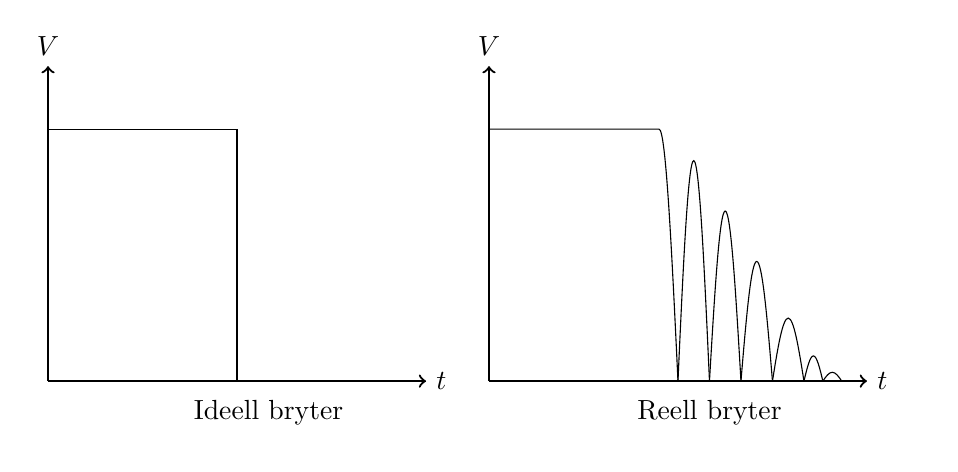
\begin{tikzpicture}[scale=0.8]

% Ideas switch
\draw[thick,->] (0,0) -- (6,0) node [right] {$t$};
\draw[thick,->] (0,0) -- (0,5) node [above] {$V$};

\draw (0,4) -- ++(3,0) -- ++(0,-4) -- ++(3,0);
\path (0,0) rectangle ++(7,-1) node [midway] {Ideell bryter};

% Realistic switch
\begin{scope}[xshift=7 cm]
\draw[thick,->] (0,0) -- (6,0) node [right] {$t$};
\draw[thick,->] (0,0) -- (0,5) node [above] {$V$};

\draw (0,4) -- ++(2.7,0) cos ++(0.3,-4);
\begin{scope}[xshift=3 cm]
\foreach \count/\top in {0/3.5,1/2.7,2/1.9,3/1}{
	\draw (\count*0.5,0) sin ++(0.25,\top) cos ++(0.25,-\top);
}
\begin{scope}[xshift=2 cm]
\foreach \count\top in {0/0.4,1/0.14}{
	\draw (\count*0.3,0) sin ++(0.15,\top) cos ++(0.15,-\top);
}
\end{scope}
\end{scope}

\path (0,0) rectangle ++(7,-1) node [midway] {Reell bryter};
\end{scope}

\end{tikzpicture}
\caption{Spenningen over en ideell- og en reell bryter.}
\label{fig::switch_bounce}
\end{figure}\\
For å komme rundt dette problemet kan man gjøre \textit{debouncing} i enten software eller hardware. I hardware ville man lagt til en RC-krets til knappen, slik at spenningen blir lavpassfiltrert før mikrokontrolleren leser den. I software kan man simpelthen vente i kort stund om man først leser en endring, slik at man hopper over transienten.\\
\\
I vårt tilfelle er knappene bare trukket høye med en pullup, og det er ikke noe vi kan gjøre for å endre på det. Siden vi i denne oppgaven koblet A-knappen direkte til LED-matrisen via GPIOTE og PPI, har vi heller ikke mulighet til å legge inn software debouncing; så her får vi bare leve med inputbounce.\\
\\
Strengt talt, kunne vi koblet knappen fra GPIOTE inn i en TIMER-instans via PPI, og deretter brukt en ny PPI-kanal til å koble en overflythendelse fra TIMER-instansen inn på GPIOTE-oppgavene, men dette er mye innsats for en marginal forbedring.

\subsection{Hint}
\begin{enumerate}
\item Husk å aktivere hver PPI-kanal. Når de er konfigurert riktig, aktiveres de ved å skrive til \mintinline{c}{CHENSET} i PPI-instansen.
\item GPIOTE-kanalene trenger ingen eksplisitt aktivering fordi \mintinline{c}{MODE}-feltet i \mintinline{c}{CONFIG}-registeret automatisk tar hånd om pinnen for dere.
\end{enumerate}

\section{Oppgave 4: Two Wire Interface}
\subsection{Beskrivelse}
En av de vanligste protokollene for seriell kommunikasjon er \mintinline{text}{I}$^2$\mintinline{text}{C} (av og til formatert som "\mintinline{text}{I2C}"), som står for \textbf{I}nter-\textbf{I}ntegrated \textbf{C}ircuit. Denne protokollen ble utviklet av Philips Semiconductor (i dag NXP Semiconductors), som naturligvis låste ned protokollen bak en del registrerte varemerker.\\
\\
Av den grunn begynte andre produsenter å implementere protokollen under et par andre navn, hvor det mest vanlige er \mintinline{text}{TWI}, som står for \textbf{T}wo \textbf{W}ire \textbf{I}nterface. Av og til kan dere også kommer over navnet \mintinline{text}{USI}, som står for \textbf{U}niversal \textbf{S}erial \textbf{I}nterface - men dette navnet er ikke like vanlig, fordi det stort sett brukes om moduler som kan operere både i \mintinline{text}{SPI}-\footnote{\textbf{S}erial \textbf{P}eripheral \textbf{I}nterface} og \mintinline{text}{I}$^2$\mintinline{text}{C}modi.\\
\\
Siden 2006 kreves det ikke lenger lisens for å implementere \mintinline{text}{I}$^2$\mintinline{text}{C} under navnet \mintinline{text}{I}$^2$\mintinline{text}{C}, men man kommer fortsatt over navn som stort sett er synonyme.\\
\\
I Nordic sitt tilfelle, implementerer nRF51serien et supersett av \mintinline{text}{I}$^2$\mintinline{text}{C}; den vanlige protokollen har støtte for vanlig rate (100 kbps) og "\textit{Fast-mode}" (400 kbps) - mens nRFen også støtter et mellommodus på 250 kbps.\\
\\
Det dere skal gjøre i denne oppgaver, er å bruke \mintinline{text}{TWI}bussen til nRF51822-SoCen til å kommunisere med akselerometeret som finnes på micro:biten. Dere skal deretter bruke denne sensorinformasjonen til å lyse opp én LED i matrisen, basert på hvordan micro:biten er orientert.

\subsection{Oppgave}
Først og fremst må dere finne ut hvordan akselerometeret er koblet til nRFen. Et naturlig sted å starte er "schematics.pdf". Det dere skal se etter er pinnene kalt \mintinline{text}{SDA} (\textbf{S}erial \textbf{Da}ta) og \mintinline{text}{SCL} (\textbf{S}erial \textbf{Cl}ock).\\
\\
Når dere vet hvordan ting er koblet opp, må dere finne ut av hva akselerometeret forventer skal skje på \mintinline{text}{TWI}bussen. Dette er beskrevet i databladet "MMA8653FC.pdf", under seksjon 5.8. Bit dere blant annet merke i hvilken adresse akselerometeret har, og hvordan dere leser ett- og flere byte.\\
\\
\warning{Ikke grav dere ned i detaljer; få et overblikk først. Om dere ikke vet hva en "start condition" er, så er det nok å vite at nRFen lager en for dere. Om dere allikevel vil vite litt mer om \mintinline{text}{I}$^2$\mintinline{text}{C}, så er appendiks \ref{appendix::i2c} stedet å lese om protokollen.}

\subsection{\texorpdfstring{\mintinline{c}{void twi_init()}}{void twi\_init()}}
Det første som må gjøres er å lage filene "twi.h" og "twi.c". I headerfilen deklarerer dere funksjonen \mintinline{c}{void twi_init()}. Den tilhørende implementasjonen skal aktivere TWI-modulen på nRFen med de riktige signallinjene og 100 kbps overføringshastighet. Legg merke til at signallinjene først må konfigureres av GPIO-modulen. Dette er beskrevet i referansemanualen, under seksjon 28.\\
\\
Som før, må dere først lage en struct som mapper ut adresseområdet til TWI-modulen, slik:
\begin{minted}{c}
#define TWI0 ((NRF_TWI_REG*)0x40003000)

typedef struct {
	volatile uint32_t STARTRX;
	[...]
} NRF_TWI_REG;
\end{minted}
Denne structen er litt større enn det UART-structen fra tidligere er. Riktige verdier for de reserverte områdene er oppgitt i hintene, men prøv først å finne dem selv.

\subsection{\texorpdfstring{\mintinline{c}{void twi_multi_read(...)}}{void twi\_multi\_read(...)}}
Som dere kan se i appendiks \ref{appendix::i2c} og i databladet til akselerometeret, er det mulig å lese- eller skrive flere byte av gangen, uten å måtte gi fra seg TWI-bussen. Dette er også mer effektivt, fordi man slipper å sende slavens adresse på nytt for hver byte. Måten I$^2$C-enheter gjør dette på, er at de automatisk hopper til et nytt internt register hver gang du har lest fra- eller skrevet til et. Dette er beskrevet i databladet.\\
\\
Istedenfor å lage funksjoner som leser- og skriver ett og ett resister, skal vi lage mer generelle funksjoner som kan lese- og skrive \textit{n} registre av gangen. Vi kan da simpelthen sette \textit{n} lik 1 om vi trenger kun ett.\\
\\
Start med å legge denne deklarasjonen i "twi.h":
\begin{minted}{c}
void twi_multi_read(
	uint8_t slave_address,
	uint8_t start_register,
	int registers_to_read,
	uint8_t * data_buffer
	);
\end{minted}
Siden vi bruker typen \mintinline{c}{uint8_t}, må vi nå inkludere \mintinline{c}{<stdint.h>} i "twi.h".\\
\\
Med denne koden ønsker vi at det følgende skal skje: Først skal vi kunne adressere en vilkårlig slave, med adresse \mintinline{c}{slave_address}. Deretter skal vi fortelle slaven hvilket register vi ønsker å begynne å lese fra; nemlig \mintinline{c}{start_register}. Når dette er gjort, skal vi lese så mange byte vi trenger (\mintinline{c}{registers_to_read}), og putte dem i et arrayet \mintinline{c}{data_buffer}. Til slutt avslutter vi kommunikasjonen og forlater TWI-bussen. Seksjon 28.6 i nRF51-databladet forklarer veldig godt hvordan dette skal gjøres.
Her har dere en oppsummering av hva som skal til:
\begin{enumerate}
\item Sett \mintinline{text}{ADDRESS}-registeret til \mintinline{c}{slave_address}.
\item Start en \textbf{skrive}operasjon.
\item Overfør \mintinline{c}{start_register} til TWI-bussen.
\item Når dere har fått \mintinline{text}{ACK} tilbake fra slaven (som betyr at en \mintinline{text}{TXDSENT}-hendelse er blitt generert), starter dere en \textbf{lese}operasjon uten å stoppe bussen. Dette kalles en \textit{repeated start sequence}.
\item Les TWI-bussen \mintinline{c}{(registers_to_read - 1)} ganger. Dette er fordi dere må sende en \mintinline{text}{NACK} til slaven den siste gangen dere leser en byte. Hver verdi dere leser, dytter dere inn i \mintinline{c}{data_buffer}.
\item Til slutt stopper dere \mintinline{text}{STOP}-oppgaven, før dere leser busser for siste gang. Dette vil gjøre at nRFen genererer en \mintinline{text}{NACK} istedenfor en \mintinline{text}{ACK}, slik at slaven ikke sender ut flere byte på bussen.
\end{enumerate}
\warning{Hendelen \mintinline{text}{TXDSENT} settes ikke automatisk til 0 når dere dytter en ny byte inn i \mintinline{text}{TXD}. Det samme gjelder også for \mintinline{text}{RXDREADY}-registeret. Derfor er det nødvendig å gjøre dette manuelt, slik:}
\begin{minted}{c}
TWI0->TXDSENT = 0;
TWI0->TXD = start_register;
while(!TWI0->TXDSENT);

[...]

TWI0->RXDREADY = 0;
TWI0->STARTRX = 1;
\end{minted}

\subsubsection{Les WHO\_AM\_I}
For å prøve ut \mintinline{c}{void twi_multi_read(...)} skal vi forsøke å lese akselerometerets enhets-ID. Denne ligger lagret i et register kalt \mintinline{text}{WHO_AM_I}. Adressen til dette registeret finner dere i seksjon 6 i databladet til akselerometeret.\\
\\
For å lage en buffer å dytte iden inn i, har vi flere alternativer. Siden vi kun er ute etter én byte, holder det å simpelthen ta pekeren til en \mintinline{c}{uint8_t}. For å gjøre det mer generelt til senere, skal vi bruke \mintinline{c}{malloc()}, som gjør det samme som \mintinline{c++}{new} gjør i C++. For å få tilgang til \mintinline{c}{malloc()}, må dere inkludere \mintinline{c}{<stdlib.h>}. For å allokere minne, gjør dere slik:
\begin{minted}{c}
uint8_t * data_buffer;
data_buffer = (uint8_t *)malloc(8 * sizeof(uint8_t));

[...]

free(data_buffer);
\end{minted}
Dette vil allokere minne til et dynamisk array av 8 \mintinline{c}{uint8_t}. Tilsvarende C++ sin \mintinline{c++}{delete}operator, bruker vi \mintinline{c}{free()} i C for å frigi dynamisk allokert minne tilbake til heapen.\\
\\
For å vite at TWI-bussen fungerer, kan dere sammenligne det dere får tilbake med akselerometerets fabrikk-ID; nemlig \mintinline{c}{0x5A}, eller 90 i base 10. Om dette er det dere får, kan dere for eksempel skru på LED-matrisen, eller sende en melding over UART for å signalisere at ting virker som det skal.\\
\\
\warning{Hver gang dere kaller \mintinline{text}{make flash}, tilbakestilles bare nRFen på micro:biten. Akselerometeret og magnetometeret lever helt sine egne liv. Det betyr at om dere sender en vanskapt TWI-meldig, kan dere sette disse i en tilstand hvor de ikke svarer på korrekte TWI-meldinger senere. Om koden deres ser riktig ut, men ting fortsatt ikke fungerer, kan dette være årsaken. Løsningen er rett og slett å ta strømmen og prøve på nytt.}

\subsection{\texorpdfstring{\mintinline{c}{void twi_multi_write(...)}}{void twi\_multi\_write(...)}}
Om dere syntes forrige deloppgave var litt vrien, er det helt forståelig. Heldigvis er det nå veldig enkelt å skrive tilsvarende funksjon for å skrive \textit{n} byte til en vilkårlig slave. Faktisk er dette enklere enn å lese, fordi vi ikke må tenke på \mintinline{text}{NACK}-grensetilfellet fra leseoperasjonen. I "twi.h" legger dere til denne deklarasjonen:
\begin{minted}{c}
void twi_multi_write(
	uint8_t slave_address,
	uint8_t start_register,
	int registers_to_write,
	uint8_t * data_buffer
	);
\end{minted}
Sekvensen vi trenger å implementere er beskrevet i seksjon 28.5 i nRF51-databladet. Sekvensen dere skal implementere, kan oppsummeres slik:
\begin{enumerate}
\item Sett \mintinline{text}{ADDRESS}-registeret.
\item Start en skriveoperasjon.
\item Skriv \mintinline{c}{registers_to_write} antall byte til bussen.
\item Kall \mintinline{text}{STOP}-oppgaven.
\end{enumerate}
Som før, må vi huske å manuelt sette \mintinline{text}{TXDSENT} til 0 etter at hendelsen er blitt aktivert:
\begin{minted}{c}
[...]

TWI0->TXDSENT = 0;
TWI0->TXD = data_buffer[n];
while(!TWI0->TXDSENT);

[...]
\end{minted}

\subsection{Les akselerometeret}
Når dere har skrevet både \mintinline{c}{twi_multi_read} og \mintinline{c}{twi_multi_write}, kan disse brukes til å lese akselerometerets X-, Y-, og Z-registre. For å slippe å kalle for mange TWI-spesifikke greier direkte fra main, har dere allerede fått utlevert en \textit{wrapper} for akselerometeret, som bruker TWI-funksjonene dere allerede har skrevet. Denne heter "accel.h" og deklarerer funksjonene \mintinline{c}{void accel_init()} og \mintinline{c}{void accel_read_x_y_z(int * data_buffer)}.\\
\\
Funksjonen \mintinline{c}{accel_init()} vil skru akselerometeret på, og sette oppdateringsraten til 200 Hz. Denne funksjonen krever at TWI-bussen er initialisert i forkant.\\
\\
Funksjonen \mintinline{c}{accel_read_x_y_z(int * data_buffer)} tar inn en peker til et array av typen \mintinline{c}{int}. Dette arrayet må minst være av størrelse 3, hvis ikke risikerer dere uforutsigbar oppførsel. Om arrayet er større en 3 har ingenting å si. Når funksjonen er kjørt ferdig, vil de tre første elementene i dette arrayet være henholdsvis X-, Y-, og Z-komponentene til akselerasjonen akselerometeret måler. Koordinatsystemet dere får komponentene i, er illustrert i figur \ref{fig::coordinate_system_accel}.

\begin{figure}[h]
\centering
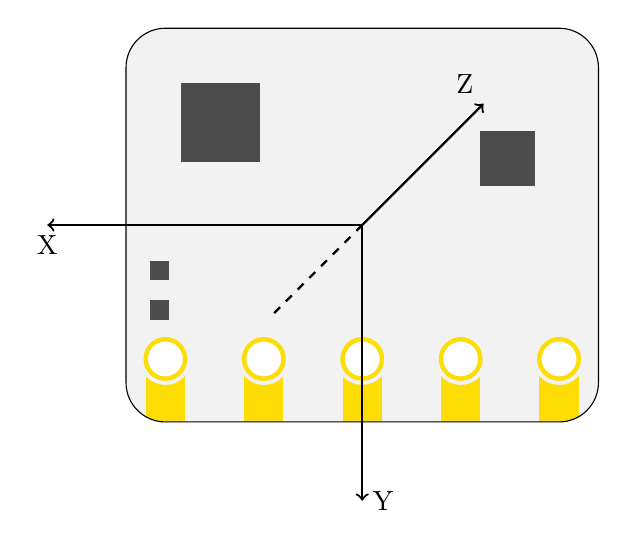
\begin{tikzpicture}
\colorlet{gold}{yellow!90!red};
\colorlet{microbit_pcb}{gray!10};
\colorlet{chip}{black!70};
\def\banana_hole_radius{0.25};
\def\microbit_rounding{0.5cm};

% micro:bit pcb layer
\fill[microbit_pcb,rounded corners=\microbit_rounding] (0,0) rectangle (6,5);

% Banana holes
\foreach \x in {0.5,1.75,...,5.5}{
\begin{scope}
\clip[rounded corners=\microbit_rounding] (0,0) rectangle (6,5);
\fill[gold] (\x - \banana_hole_radius, 0.8) rectangle (\x + \banana_hole_radius, 0);
\fill[microbit_pcb] (\x, 0.8) circle [radius=\banana_hole_radius + 0.08];
\end{scope}
\draw[gold,ultra thick,fill=white] (\x, 0.8) circle [radius=\banana_hole_radius];
}

% Processor
\begin{scope}[xshift=0.7cm,yshift=3.3cm]
\def\w{1}
\fill[chip] (0,0) rectangle (\w,\w);
\end{scope}

% Interface
\begin{scope}[xshift=4.5cm,yshift=3cm]
\def\w{0.7}
\fill[chip] (0,0) rectangle (\w,\w);
\end{scope}

% Magnetometer
\begin{scope}[xshift=0.3cm,yshift=1.8cm]
\def\w{0.25}
\fill[chip] (0,0) rectangle (\w,\w);
\end{scope}

% Accelerometer
\begin{scope}[xshift=0.3cm,yshift=1.3cm]
\def\w{0.25}
\fill[chip] (0,0) rectangle (\w,\w);
\end{scope}

% micro:bit border
\draw[rounded corners=\microbit_rounding] (0,0) rectangle (6,5);

% Coordinate system
\draw[thick,->] (3,2.5) -- ++(0,-3.5) node [right] {Y};
\draw[thick,->] (3,2.5) -- ++(-4,0) node [below] {X};
\draw[thick,->] (3,2.5) -- ++(0,0,-4) node[above left] {Z};
\draw[thick,dashed] (3,2.5) -- ++(0,0,3);
\end{tikzpicture}
\caption{Høyrehåndskoordinatsystemet \mintinline{c}{accel_read_x_y_z} bruker.}
\label{fig::coordinate_system_accel}
\end{figure}

\subsubsection{Fyll inn konstanter i accel.c}
Før dere kan kan bruke funksjonene i "accel.h", må dere fylle ut tre verdier i implementasjonsfilen "accel.c":
\begin{itemize}
\item \mintinline{text}{ACCEL_ADDR} skal være adressen til akselerometeret, som dere fant i databladet "MMA8653FC.pdf" under seksjon 5.8.
\item \mintinline{text}{ACCEL_DATA_REG} skal være adressen til det mest signifikante bytet av akselerometerets X-komponent. Dette kan dere finne under seksjon 6 i databladet.
\item \mintinline{text}{ACCEL_CTRL_REG_1} skal være adressen til registeret som kontrollerer dataraten, og om akselerometeret er på eller ei. Dette kan også finnes under seksjon 6 i databladet.
\end{itemize}

\subsubsection{Skriv verdier til skjerm via UART}
Når dere har fylt inn konstantene i "accel.c", er det fritt frem for å bruke funksjonene filen definerer. For å gjøre det lett å skrive ting til skjermen, har dere også fått utlevert "utility.h" med tilhørende implementasjonsfil. Denne filen gir dere funksjonen \mintinline{c}{utility_print}, som etterligner funksjonaliteten til \mintinline{c}{printf}, uten å trekke inn for mye annet søl som \mintinline{c}{<stdio.h>} rasker med seg.\\
\\
Dere velger selv om dere vil bruke \mintinline{c}{utility_print}, men her har dere iallefall et eksempel på hvordan funksjonen kan brukes:
\begin{minted}{c}
int * data_buffer = (int *)malloc(3 * sizeof(int));
accel_read_x_y_z(data_buffer);

int x_acc = data_buffer[0];
int y_acc = data_buffer[1];
int z_acc = data_buffer[2];

utility_print(&uart_send, "X: %6d Y: %6d Z: %6d\n\r", x_acc, y_acc, z_acc);
\end{minted}
Dette er også dokumentert i filen "utility.h".


\subsection{Lys opp riktig diode}
Når dere greier å lese fra akselerometeret, er det duket for å ha det litt gøy med LED-matrisen til micro:biten. På grunn av den litt artige måten matrisen er koblet opp på, er det litt styr å skru på én og én diode. For å skjerme dere for å måtte skrive grisete kode selv, har dere fått utlevert filen "ubit\_led\_matrix.h", som dere er mer enn velkomne til å benytte dere av. Et forslag til hvordan denne brukes, ser slik ut:
\begin{minted}{c}
ubit_led_matrix_init();

[...]

// Calculate X-LED and Y-LED from accelerometer reading

ubit_led_matrix_light_only_at(x_led, y_led);
\end{minted}
Koordinatsystemet \mintinline{c}{ubit_led_matrix_light_only_at(int x, int y)} bruker, er illustrert i figur \ref{fig::coordinate_system_led_matrix}.
\begin{figure}[ht]
\centering
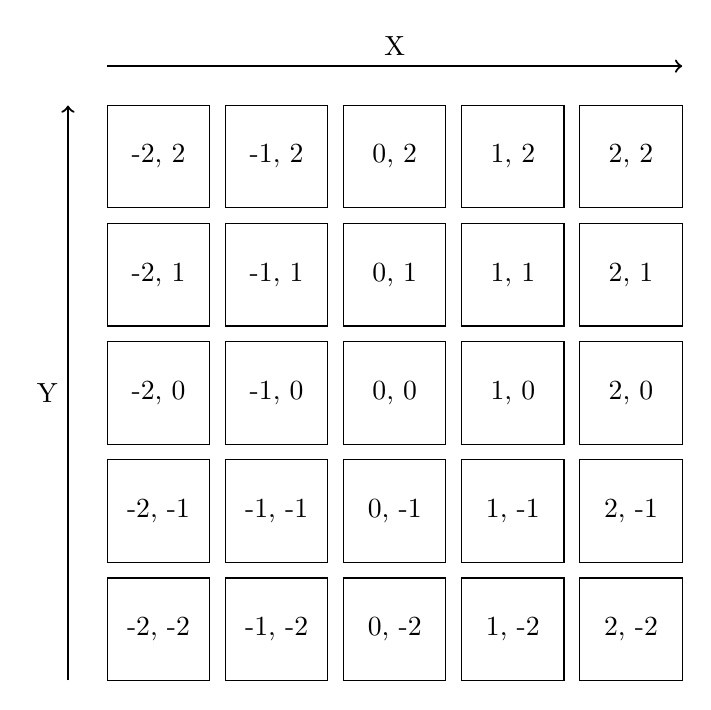
\begin{tikzpicture}
\foreach \x in {0,1,...,4}{
\foreach \y in {0,1,...,4}{
\pgfmathtruncatemacro{\xlabel}{\x-2}
\pgfmathtruncatemacro{\ylabel}{\y-2}
\draw (\x * 1.5,\y * 1.5) rectangle ++(1.3,1.3) node [midway] {\xlabel, \ylabel};
}
}
\draw[thick,->] (0,7.3 + 0.5) -- ++(7.3,0) node [midway, above] {X};
\draw[thick,->] (-0.5, 0) -- ++(0, 7.3) node [midway, left] {Y};
\end{tikzpicture}
\caption{Koordinatsystemet \mintinline{c}{ubit_led_matrix_light_only_at} bruker.}
\label{fig::coordinate_system_led_matrix}
\end{figure}
Hvordan dere regner ut hvilke koordinater som skal lyse opp gitt akselerasjon i x- og y-retning, er opp til dere. Om dere vil gjøre det enkelt, har dere en ganske rett frem metode her:
\begin{minted}{c}
int x_accel = data_buffer[0];
int y_accel = data_buffer[1];

int x_dot = x_accel / 50;
int y_dot = - y_accel / 50;

ubit_led_matrix_light_only_at(x_dot, y_dot);
\end{minted}

\subsection{Frivillig: Les magnetometeret}
Med \mintinline{c}{void twi_multi_read(...)} og \mintinline{c}{void twi_multi_write(...)} er det en smal sak å lese fra magnetometeret også. Dette gjøres stort sett på samme måte som for akselerometeret, og er beskrevet i databladet "MAG3110.pdf". Hva dere gjør med det, er opp til dere - men å bruke det som kompass er jo det åpenbare alternativet.

\subsection{Hint}
\begin{enumerate}
\item Verdier for de 15 reserverte områdene: 1, 2, 1, 56, 4, 1, 4, 49, 63, 110, 14, 1, 2, 1, 24.
\item nRF51822en har to instanser av TWI-modulen, som betyr at dere kan ha to forskjellige TWI-linjer oppe på en gang. Vi trenger bare den ene.
\item Husk å manuelt sette \mintinline{text}{RXDREADY} og \mintinline{text}{TXDSENT} til 0 etter at dere sjekker disse registrene.
\item Det er egentlig unødvendig å bruke dynamisk minne i denne oppgaven. Siden vi vet ved \textit{compile time} hvor stor plass vi trenger, kan vi simpelthen opprette et vanlig array. Vi bruker dynamisk minne bare for å eksponere dere til C-ekvivalenten av \mintinline{c++}{new} ;)
\end{enumerate}

\section{Oppgave 5: Pulsbreddemodulasjon}
\subsection{Beskrivelse}
Pulsbreddemodulasjon er en modulasjonsteknikk hvor man gir et signal en satt periode, og varierer hvor lenge signalet er høyt i løpet av denne perioden. Dette kalles modulasjonens \textit{duty cycle} og er illustrert i figur \ref{fig::pwm_illustration}. Pulsbreddemodulasjon er utbredt i dag, og det sies ofte at pulsbreddemodulasjon (PWM) var til frekvensmodulasjon (FM), slik som frekvensmodulasjon var til amplitudemodulasjon (AM) - altså en ganske grom forbedring, da teknologien var ny.
\begin{figure}[h]
\centering
\begin{tikzpicture}
%\usetikzlibrary{decorations.pathreplacing};
\draw[thick] (0,0) -- ++(0,3) -- ++(2,0) -- ++(0,-3) -- ++(3,0) -- ++(0,3) -- ++(1,0) -- ++(0,-3) -- ++(4,0);
\draw[dashed] (0,0) -- ++(0,4);
\draw[dashed] (5,0) -- ++(0,4);
\draw[dashed] (10,0) -- ++(0,4);
\draw[decorate,decoration={brace,amplitude=5pt,mirror,raise=5pt}] (0,0) -- ++(2,0) node [midway,below=10pt] {40 \% duty cycle};
\draw[decorate,decoration={brace,amplitude=5pt,mirror,raise=5pt}] (5,0) -- ++(1,0) node [midway,below=10pt] {20 \% duty cycle};
\draw[decorate,decoration={brace,amplitude=5pt,raise=5pt}] (0,4) -- ++(5,0) node [midway,above=10pt] {Periode};
\end{tikzpicture}
\caption{Illustrasjon av pulsbreddemodulasjon.}
\label{fig::pwm_illustration}
\end{figure}\\
Om noen av dere har vært borti andre mikrokontrollere, som en AVR, eller storebroren til vår mikrokontroller; en nRF52 - da har dere nok blitt bortskjemt med eget dedikert hardware for pulsbreddemodulasjon. Det er egentlig ganske vanlig, og gjør ting mye enklere for oss. Så heldige er vi dessverre ikke, når det kommer til nRF51-serien.\\
\\
For å finne en kreativ løsning på denne knipen, kunne vi prøvd å lage pulsbreddemodulasjon i software. Dette er en dårlig løsning, fordi vi da må vite hvor fort hver del av koden vår kjører, og passe på at vi ikke endrer den når ting funker. Om man så blander inn \textit{interrupts} vil man plutselig være helt i villrede igjen.\\
\\
En bedre løsning er å bruke en \mintinline{text}{TIMER}-modul til å generere perioden og en satt \textit{duty cycle}, \mintinline{text}{GPIOTE} til å skru en pinne på og av, og \mintinline{text}{PPI} til å koble de to modulene sammen sånn at CPUen kan leve sitt eget liv. Dette vil fungere strålende, men er fortsatt ikke helt trivielt å få til. Derfor har vi skrevet en del av koden for dere, men dere må fortsatt finne ut av noen verdier som skal settes på egenhånd.\\
\\
Når dette er gjort skal dere koble det genererte signalet inn på en servomotor for å kontrollere rotasjonen dens.

\subsection{Oppgave}
Dere skal bruke den utleverte funksjonen \mintinline{c}{void pwm_init(...)} til å konfigurere et pulsbreddemodulert signal på nRFens pinne 20. Dette svarer til pinne 12 på det rød brødbrettadapteren dere har fått utdelt. Funksjonen vil benytte seg av \mintinline{text}{PPI}-kanal 0, 1, 2, og 3, samt \mintinline{text}{TIMER}-instans 1, og \mintinline{text}{GPIOTE}-kanal 0. Dermed er det sikkert lurt å unngå å bruke disse i egen kode mens dere pulsbreddemodulerer.\\
\\
\mintinline{c}{void pwm_init(int prescaler, int period, int init_duty)} vil først og fremst bestemme frekvensen til \mintinline{text}{TIMER1}, ut fra formel \ref{eq::pwm_frequency}. Når frekvensen til \mintinline{text}{TIMER1} er bestemt, vil den inkrementere et sammenligningsregister ved hver klokkepuls. Når dette registeret når verdien \mintinline{c}{period}, vil registeret tilbakestilles. Verdien \mintinline{c}{init_duty} - som må være mindre enn \mintinline{c}{period}, vil bestemme hvor lenge signalet skal være høyt.
\begin{equation}
f_\mathrm{TIMER} = \frac{16\,\mathrm{MHz}}{2^{\mathrm{prescaler}}}
\label{eq::pwm_frequency}
\end{equation}
Altså, om dere setter \mintinline{c}{prescaler} til 9 - som er den høyeste verdien tillatt, vil frekvensen til \mintinline{text}{TIMER1} være 31250 Hz. Om dere da setter \mintinline{c}{period} til 31250, og \mintinline{c}{init_duty} til 15625; vil dere ende opp med et signal som har 50 \% duty cycle, og 1 sekund periode.\\
\\
Dere skal lage et signal som har 20 ms periode, og pulsbredde på 1,5 ms. Hvilken prescaler dere bruker er opp til dere, men den må ligge i intervallet $[0,9]$. Lavere prescaler vil gi høyere klokkeoppløsning, men øke strømforbruket til \mintinline{text}{TIMER1}.\\
\\
Når dere har laget signalet, sjekker dere med et oscilloskop for å bekrefte at ting fungerer som det skal.

\subsection{Sett duty cycle fra akselerometer}
Når dere greier å lage et pulsbreddemodulert signal, skal vi endre duty cyclen basert på hvordan akselerometeret holdes. Et forslag er å ta utgangspunkt i akselerometerets X-akselerasjon. Dere skal så oversette denne målingen til en pulsbredde mellom 1,0 ms til 2,0 ms - der 1,5 ms betyr at akselerometeret holdes plant.\\
\\
I tilfelle dere er har glemt hvordan man kan gjøre en sånn oversetting, er det lurt å lese seksjon \ref{sec::convert_f_to_c}. Ellers er det bare å skippe glatt over.

\subsubsection{Konvertering mellom Fahrenheit og Celsius}
\label{sec::convert_f_to_c}
Celsius er en grei temperaturskala som brukes i den siviliserte verden. Uheldigvis insisterer USA, Belize, Palau, Bahamas og Caymanøyene på en være en gjeng vrangpåler - som gjør konvertering til Fahrenheit nødvendig.\\
\\
I Celsius fryser vann ved $0^\circ\mathrm{C}$, og koker ved $100^\circ\mathrm{C}$. I Fahrenheit fryser vann derimot ved $32^\circ\mathrm{F}$, og koker ved $212^\circ\mathrm{F}$. Vi kan da definere noen konstanter i ligning \ref{eq::temp_constants}:
\begin{equation}
y_0 = 32\qquad y_1 = 212\qquad x_0 = 0\qquad x_1 = 100
\label{eq::temp_constants}
\end{equation}
Her svarer $y$ til Fahrenheit, og $x$ til Celsius. Deretter kverner vi disse simpelthen gjennom ligning \ref{eq::points_to_slope}:
\begin{equation}
(y - y_0) = \frac{y_1 - y_0}{x_1 - x_0}\bigg(x - x_0\bigg)
\label{eq::points_to_slope}
\end{equation}
Når det er gjort, ender vi opp med relasjonen $y = 1.8 x + 32$, som er formelen for Celsius $\rightarrow$ Fahrenheit (eller motsatt, fordi ligningen er invertibel). Dette kan brukes på samme måte for å oversette akselerometermåling til pulsbredde.

\subsection{Styr servomotoren}
Før dere begynner å leke med servomotoren, kobler dere på oscilloskopet igjen, og bekrefter at det ikke er mulig å komme utenfor en pulsbredde på 0,9 ms til 2,1 ms - uansett hvordan dere vrir og vrenger på micro:biten. Hvis dere går utenfor dette området er det nemlig lett å brenne opp servomotoren.\\
\\
Når dere er sikre på at signalet er riktig, kobler dere brun ledning fra servomotoren til jord; rød til 3,3 V, og oransje til pulsbreddesignalet. Nå skal servomotoren kjøre frem og tilbake avhenging av hvordan dere orienterer micro:biten.

\subsubsection{Artig motoroppførsel?}
Det kan hende at servomotoren kjører fint i én retning, men "hakker" i den andre - eller at oppførselen generelt virker litt sporadisk - selv om oscilloskopet bekreftet at dere har gjort ting rett.\\
\\
Det er helt normalt og kommer av at micro:biten egentlig ikke er dimensjonert for å drive en servo - selv om dette er den minst ressurskrevende servomotoren på DigiKey$^{\tiny{\textregistered}}$.\\
\\
Hvis dere ønsker bedre oppførsel har dere jo fått brødbrettet - så her er det bare å legge inn en transistor, optocoupler, level converter, eller noe lignende.




\newpage
\appendix
\section{Bitoperasjoner i C}
\label{appendix::bitoperations}
Når vi arbeider med mikrokontrollere er vi stort sett ikke veldig langt unna "metallet", i den forstand at vi hele tiden loker rundt med registre og individuelle bit for å oppnå det vi vil. C er et godt egnet språk for mikrokontrollere, nettopp fordi det ikke gjemmer bort tilgang til slike plattformspesifikke detaljer.\\
\\
C har seks forskjellige bitoperatorer:
\begin{itemize}
\item[\mintinline{c}{&}] Bitvis og (AND)
\item[\mintinline{c}{|}] Bitvis eller (OR)
\item[\mintinline{c}{^}] Bitvis eksklusiv eller (XOR)
\item[\mintinline{c}{~}] Ens komplement (Flipp alle bit)
\item[\mintinline{c}{<<}] Venstreskift
\item[\mintinline{c}{>>}] Høyreskift
\end{itemize}
Den beste måten å lære seg disse på, er nok å tegne opp noen byte og gjøre operasjonene for hånd med penn og papir et par ganger. Her har dere noen eksempler:
\begin{minted}{c}
// The prefix 0b means "number in binary"
uint8_t a = 0b10101010;
uint8_t b = 0b11110000;
uint8_t c;

c = a | b;        // c is now 1111 1010
c = a & b;        // c is now 1010 0000
c = b >> 2;       // c is now 0011 1100
c = a ^ b;        // c is now 0101 1010
c = ~b;           // c is now 0000 1111
\end{minted}
Som de andre operatorene, er det mulig å kombinere en bitvis operasjon og et likhetstegn for å modifisere et tall direkte:
\begin{minted}{c}
uint8_t a = 0b10101010;

a <<= 4;          // a is now 1010 0000
a >>= 4;          // a is now 0000 1010
a |= (a << 4);    // a is now 1010 1010
a |= (a >> 1);    // a is now 1111 1111
a &= ~(a << 4);   // a is now 0000 1111
\end{minted}
\warning{Som dere kanskje ser, er vestreskift det samme som å multiplisere med 2, og høyreskift det samme som å dividere på 2. Ikke finn på å bytte ut multiplikasjon og divisjon med 2, med venstre- og høyreskift i "vanlig" kode. Det vil bare gjøre ting lite leselig - og dette er uansett en optimalisering en vanlig kompilator gjør for dere.}\\
\\
\\
I C bruker vi tall som boolske verdier, der vi tolker 0 som \mintinline{c}{false} og alt annet som \mintinline{c}{true}. Det betyr at vi kan isolere et eneste bit, og så teste for sannhet på vanlig vis om vi foreksempel ønsker å vite om en knapp er trykket inne:
\begin{minted}{c}
// GPIO->IN is a register of 32 bits, and button A is held if
// the 17th bit is zero (zero-indexed)

int ubit_button_press_a(){
	return (!(GPIO->IN & (1 << 17)));
}

// (1 << 17) gets us bit number 17, counting from 0
// & isolates the 17th bit in GPIO->IN, because we do an AND
// operation with a single bit masking.
// We finally negate the answer, to return true if the bit
// was not set.
\end{minted} 

\section{\texorpdfstring{Kort om I$^2$C (a.k.a. TWI)}{Kort om I2C (a.k.a. TWI)}}
\label{appendix::i2c}
I$^2$C (eller bare I2C) er en av de vanligste bussprotokollene for innvevde datasystemer der ute. Det finnes mange andre, slik som SPI, CAN, Ethernet, RS-232/422/485, 1-wire, etc.\\
\\
Den store fordelen ved I$^2$C er derimot at den er ekstremt simpel, billig å implementere, og støttes av nesten alt. Den er en ganske treg protokoll, med maks overføringshastighet på 400 kbps, men dette er mer enn nok for et par sensorer koblet til en mikrokontroller.\\
\\
Oppkoblingen av en I$^2$C-buss ser dere illustrert i figur \ref{fig::i2c::connection}. Dette er en såkalt \textit{open-drain} buss, fordi enheter koblet til bussen bare kan trekke de to signallinjene lave. Linjene trekkes høye når bussen ikke er i bruk av et sett med pullupmotstander.
\begin{figure}[h]
\centering
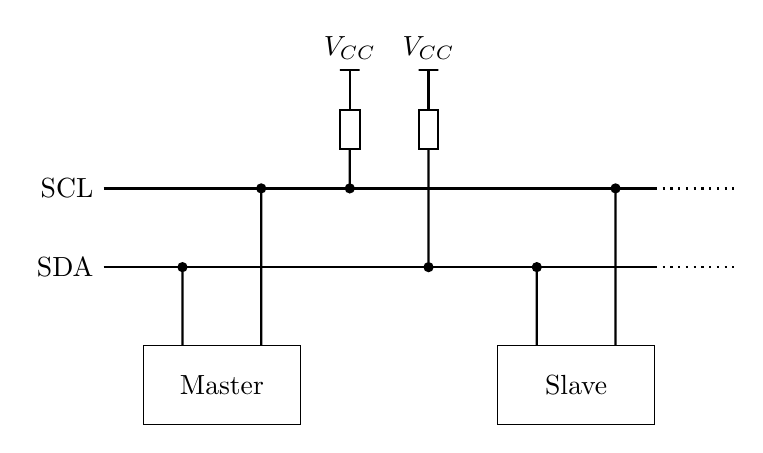
\begin{tikzpicture}
\draw[thick] (0,3) node [left] {SCL} -- ++(7,0);
\draw[thick, dotted] (7,3) -- ++(1,0);
\draw[thick] (0,2) node [left] {SDA} -- ++(7,0);
\draw[thick, dotted] (7,2) -- ++(1,0);

\begin{scope}[xshift=3cm,yshift=3.5cm,thick]
\draw (0,0) rectangle ++(0.25,0.5);
\draw (0.125,0.5) -- ++(0,0.5) -- ++(-0.125,0) -- ++(0.25,0) -- ++ (-0.125,0) node [above] {$V_{CC}$};
\filldraw (0.125,0) -- ++(0,-0.5) circle [radius=0.05];
\end{scope}

\begin{scope}[xshift=4cm,yshift=3.5cm,thick]
\draw (0,0) rectangle ++(0.25,0.5);
\draw (0.125,0.5) -- ++(0,0.5) -- ++(-0.125,0) -- ++(0.25,0) -- ++ (-0.125,0) node [above] {$V_{CC}$};
\filldraw (0.125,0) -- ++(0,-1.5) circle [radius=0.05];
\end{scope}

\begin{scope}[xshift=0.5cm,yshift=0]
\draw (0,0) rectangle ++(2,1) node [midway] {Master};
\filldraw[thick] (0.5, 1) -- ++(0,1) circle [radius=0.05];
\filldraw[thick] (1.5, 1) -- ++(0,2) circle [radius=0.05];
\end{scope}

\begin{scope}[xshift=5cm,yshift=0]
\draw (0,0) rectangle ++(2,1) node [midway] {Slave};
\filldraw[thick] (0.5, 1) -- ++(0,1) circle [radius=0.05];
\filldraw[thick] (1.5, 1) -- ++(0,2) circle [radius=0.05];
\end{scope}
\end{tikzpicture}
\caption{Oppkobling av en I$^2$C-buss.}
\label{fig::i2c::connection}
\end{figure}
\\
Protokollen støtter flere enn én master på samme buss, og enheter kan legges til eller fjernes uten å påvirke de andre enhetene som deler bussen. Faktisk kan man i teorien legge til vilkårlig mange enheter - men vanlig I$^2$C støtter kun 112 unike adresser\footnote{7-bits adresse gir 128 mulige varianter, men enkelte adresser er reservert. I$^2$C har også et utvidet 10-bits adressesystem, som øker adresseområdet til litt over tusen enheter.}. Om man av en eller annen grunn trenger flere enn dette, blir det nødvendig å gjøre litt triksing, eller bruke en annen bussprotokoll.
\subsection*{Start condition}
Når bussen ikke er i bruk, er både SCL og SDA høye. En overføring startes ved at en master (av potensielt mange) genererer en \textit{start condition} på busslinjene. En \textit{start condition} betyr simpelthen at masteren trekker SDA lav, etterfulgt av SCL.\\
\\
Når begge linjene er trukket lave, vil masteren sette første databit på SDA, før SCL går høy for å signalisere til slavene på bussen at SDA kan leses. Etter dette er overføringen i gang. En start condition er illustrert i figur \ref{fig::i2c::start_condition}.
\begin{figure}[h]
\centering
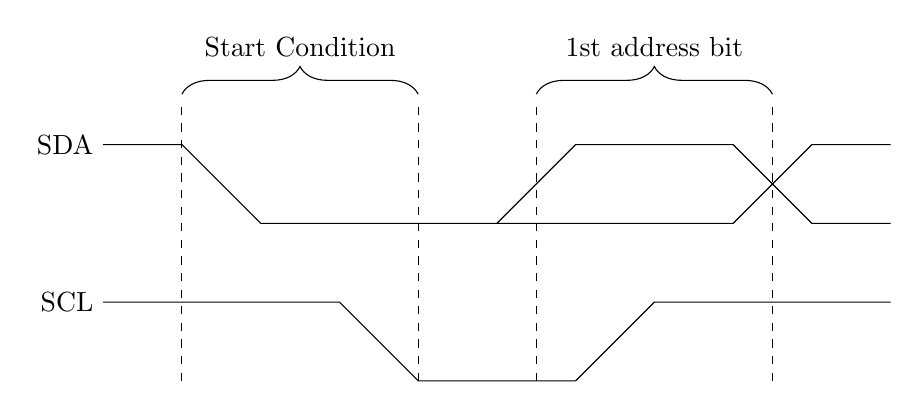
\begin{tikzpicture}
%\usetikzlibrary{decorations.pathreplacing}
\draw (0,3) node [left] {SDA} -- ++(1,0) -- ++(1,-1) -- ++(3,0) -- ++(1,1) -- ++(2,0) -- ++(1,-1) -- ++(1,0) ++ (0,1) -- ++(-1,0) -- ++(-1,-1) -- ++(-3,0);
\draw (0,1) node [left] {SCL} -- ++(3,0) -- ++ (1,-1) -- ++(2,0) -- ++(1,1) -- ++(3,0);
\draw[dashed] (4,0) -- ++(0,3.5);
\draw[dashed] (1,0) -- ++(0,3.5);
\draw[decorate,decoration={brace,amplitude=10pt,raise=4pt}] (1,3.5) -- ++(3,0) node [midway, above=0.5cm] {Start Condition};
\draw[dashed] (5.5,0) -- ++(0,3.5);
\draw[dashed] (8.5,0) -- ++(0,3.5);
\draw[decorate,decoration={brace,amplitude=10pt,raise=4pt}] (5.5,3.5) -- ++(3,0) node [midway, above=0.5cm] {1st address bit};
\end{tikzpicture}
\caption{Start condition, og første adressebit, på I$^2$C-buss.}
\label{fig::i2c::start_condition}
\end{figure}
\subsection*{Overføring}
For hvert bit som overføres, må det være riktig på SDA i det SCL går fra lav til høy. Hver slave taster SDA-linjen for hver stigende flanke på SCL-linjen. Begge linjene styres i utgangspunktet av masteren, men hvis en slave ikke er i stand til å motta flere bit, kan den tvinge masteren til å avvente videre sending ved å trekke SCL lav. Dette kalles \textit{clock stretching}.\\
\\
Hver byte overført over I$^2$C må bekreftes av en mottaker. Man sier gjerne at mottakeren sender en "ACK" (for \textbf{ack}nowledgement) tilbake. Dette gjøres ved at masteren slipper SDA-linjen etter det åttende bitet den har sendt. Deretter vil masteren generere en ekstra klokkepuls på SCL; og nå er det opp til mottakeren å trekke SDA lav for å signalisere at den har mottatt bytet. Hvis masteren ikke merker at SDA trekkes lav, vil den avbryte sendingen.

\subsection*{Adressering}
Som sagt kan en I$^2$C-buss være vert for mange enheter. For å signalisere hvilken enhet masteren ønsker å snakke med, vil hver enhet ha en unik adresse på bussen. For sensorer (slik som akselerometeret og magnetometeret på micro:biten) vil adressen stort sett være forhåndsbestemt fra fabrikanten uten mulighet til å endres.\\
\\
Etter at en start condition er blitt generert, vil det første bytet masteren sender bestå av 7 adressebit, og ett retningsbit. Retningsbitet forteller om masteren ønsker å skrive til-, eller lese fra en mottaker. Retningsbitet vil være 1 for en leseoperasjon, og 0 for en skriveoperasjon.\\
\\
Så fremst 10-bits adressering ikke brukes, vil alle byte som følger etter dette første bytet, være data.

\subsection*{Arbitrering}
Hvis det finnes flere mastere på en buss, kan det hende at to mastere griper etter I$^2$C-linjene samtidig. For å bli enige om hvem som får lov til å sende først, brukes mottakeradressen som meglingsmiddel.\\
\\
I$^2$C er en såkalt CSMA/CD-protokoll (\textbf{C}arrier \textbf{S}ense \textbf{M}ultiple \textbf{A}ccess with \textbf{C}ollision \textbf{D}etection), som rett og slett betyr at hver I$^2$C-master vil selv sjekke etter busstilstanden og sammenligne med det den forventer.\\
\\
Hvis to mastere begynte en overføring samtidig, og en av dem ønsket å sende et høyt bit, mens den andre ønsket å sende et lavt bit - vil masteren som sende det lave bitet trekke SDA lav. Dette vil masteren som ønsket å sende et høyt bit merke, og dermed avslutte sendingen. Fordi adressebytet sendes først, vil den masteren som adresserer den laveste adressen vinne (så lenge de ikke snakker til samme adresse).

\subsection*{Tungetrim}
I$^2$C er en CSMA/CD-protokoll. En annen utbredt protokoll, kalt CAN (\textbf{C}ontroller \textbf{A}rea \textbf{N}etwork) - som brukes veldig mye i bilindustrien - er en såkalt CSMA/CD+AMP-protokoll.\\
\\
Forkortelsen CSMA/CD+AMP står for "\textbf{C}arrier \textbf{S}ense \textbf{M}ultiple \textbf{A}ccess with \textbf{C}ollision \textbf{D}etection and \textbf{A}rbitration by \textbf{M}essage \textbf{P}riority".\\
\\
Grunnen til det lange navnet er antagelig at Bosch (Skaperene av CAN) ønsket en effektiv promillekontroll i samme slengen; greier du å uttale remsen uten å snakke utydelig - ja, da er du nok kjørbar også ;)

\end{document}